%
% Suitability and Application
% Jason Brownlee
%
\chapter{Suitability and Application}
\label{chap:iidle}

%
% Overview
% Provides an overview of the chapter and its structure, and a description of what is intended to be achieved by providing this documentation. A description of why and how this chapter follows on from the previous chapter
%
\section{Chapter Overview}
\label{sec:iidle:overview}
% setting the scene
The previous chapters proposed and investigated models and algorithms inspired by clonal selection with little regard for their applicability as Computational Intelligence tools. Before applicability is considered, it is important to outline a systematic methodology to define suitability not just for the application of a technique to a problem, but also for comparison of a technique to other similar techniques as well as the transferability of results on one problem to other similar problems.
% this chapter
Section~\ref{sec:iidle:suitability} considers the suitability of application of the clonal selection algorithms. A simple feature-based suitability methodology is defined and is applied to the base algorithms from across the three paradigms both eliciting general features and projecting those features onto general attributes of computational problems.
% examples
Two problem formalisms that embody many of the most difficult problems faced by Artificial and Computational Intelligence are reviewed: Function Optimisation in Section~\ref{sec:iidle:function:optimization} and Function Approximation in Section~\ref{sec:iidle:function:approximation}. Each formalism is described in terms of (1) its general properties, (2) a set of specialised sub-problems, and (3) select approaches from the fields of AI and CI that both address problem instances that fit into the formalism and exhibit some superficially similar features with clonal selection algorithms from across the hierarchical framework. These problem examples provide a tangible framing for the features of the clonal selection algorithms, which are systematically mapped onto specific and \emph{suitable} sub-problems from the respective problem domains.

%
% Suitability of Application
%
\section{Suitability of Application}
\label{sec:iidle:suitability}
% utility as problems solvers
From a problem-solving perspective, the tools that emerge from the field of Computational Intelligence are generally assessed with regard to their utility as \emph{efficiently} or \emph{effectively} solving problems.
% nfl
An important lesson from the `no-free-lunch theorem' was to \emph{bound claims of applicability} (Section~\ref{subsec:methodology:experimental}). An approach toward this end is to consider the suitability of a given strategy with regard to the feature overlap with the attributes of a given problem domain. From a Computational Intelligence perspective, one may consider the architecture, processes, and constraints of a given strategy as the features of an approach. 
% focus of this section
This section lists such features of the approaches from the Cellular, Tissue, and Host Paradigms and projects their features onto general capability with regard to problem features to which the approaches may be suitable. These so-called general features provide the foundation for further consideration of the application of the clonal selection algorithms from across the hierarchical framework. System features are discussed in the context of the general intention and observed behaviours. Paradigms are discussed in a compressed form, not taking into consideration the subsumed properties of the hierarchical framework.

%
% Considering Suitability
% 
\subsection{Considering Suitability}
\label{sec:iidle:suitability:framework}
% properties
In this work, the suitability of the application of an `approach' to a `problem' takes into considerations concerns such as the \emph{appropriateness} (can the approach address the problem), the \emph{feasibility} (available resources and related efficiency concerns), and the \emph{flexibility} (ability to address unexpected or unintended effects).
% my approach
This section summarises a general methodology toward addressing the problem of suitability in the context of Computational Intelligence tools. This methodology involves (1) the systematic elicitation of system and problem features, and (2) the consideration of the overlap of problem-problem, algorithm-algorithm, and problem-algorithm overlap of feature sets. 

%
% Systematic Feature Elicitation
%
\subsubsection{Systematic Feature Elicitation}
A \emph{feature} of a system (tool, strategy, model) or a problem is a distinctive element or property that may be used to differentiate it from similar and/or related cases. Examples may include functional concerns such as: processes, data structures, architectures, and constraints, as well as emergent concerns that may have a more subjective quality such as general behaviours, organisations, and higher-order structures. The process of the elicitation of features may be taken from a system or problem perspective as follows:

\begin{itemize}
	\item \emph{System Perspective}: This requires a strong focus on the lower level functional elements and investigations that work toward correlating specific controlled organisations towards predictable emergent behaviours. An example is the central focus of this work in Chapters \ref{chap:cells} through \ref{chap:framework}.
	\item \emph{Problem Perspective}: May require both a generalisation of the specific case to the general problem case, as well as a functional or logical decomposition into constituent parts.
\end{itemize}

Problem \emph{generalisation} and \emph{functional decomposition} are important and well used patterns for problem solving in the broader fields of Artificial Intelligence and Machine Learning as the promotion of simplification and modularity can reduce the cost and complexity of achieving solutions \cite{Russell1995, Brooks1986}.

%
% Feature Overlap
%
\subsubsection{Feature Overlap}
% general overlap
Overlap in elicited features may be considered from three important perspectives: \emph{between systems}, \emph{between problems}, and \emph{between a system and a problem} (depicted in Figure~\ref{fig:problem-strategy-suitability}). Further, such overlap may be considered at different levels of detail with regard to generalised problem solving strategies and problem definitions.
% cases
These overlap cases are considered as follows:

\begin{itemize}
	\item \emph{System Overlap}: Defines the suitability of comparing one system to another, referred to as \emph{comparability}. For example, systems may be considered for the same general problems and compared in terms of theoretical or empirical capability, the results of which may only be meaningful if the systems are significantly similar to each other as assessed in terms of feature overlap. 
	\item \emph{Problem Overlap}: Defines the suitability of comparing one problem to another, referred to as \emph{transferability}. From a systems focus for example, transferability refers to the capability of a technique on a given problem to be transferred to another problem, the result of which is only meaningful if there is a strong overlap between the problems under consideration.
	\item \emph{System-Problem Overlap}: Defines the suitability of a system on a given problem, referred to as \emph{applicability}. For example, a system is considered suitable for a given problem if it has a significant overlap in capabilities with the requirements of the problem definition.
\end{itemize}


\begin{figure}[htp]
	\centering
		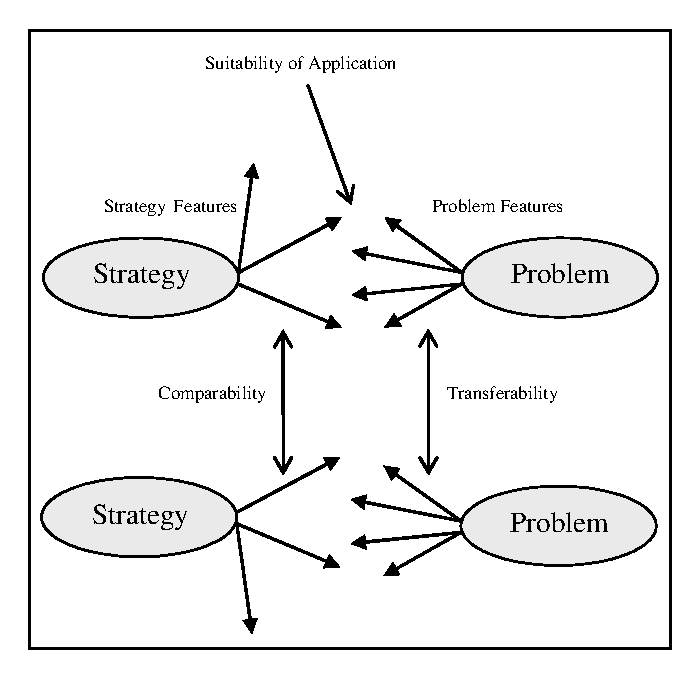
\includegraphics[scale=0.75]{IIDLE/problem-strategy-suitability}
	\caption{Depiction that the suitability of application of a strategy to a problem is defined by the overlap in their features, as well as the comparability with other strategies, and transferability of results to other problems.}
	\label{fig:problem-strategy-suitability}
\end{figure}

% noise
Such mappings are expected to have noise given the subjective assessment and/or complexity required in both the elicitation and consideration overlap of the of features, the noisiest of which is expected to be the mapping between systems and problems. 
% nfl
The mapping of salient features of algorithms and problems was proposed as an important reconciliation of the `no-free-lunch theorem' by Wolpert and Macready \cite{Wolpert1997}, although the important difference of this approach is that the system and algorithm are given prior to the assessment. In \cite{Wolpert1995}, Wolpert and Macready specifically propose the elicitation of the features from a problem first perspective, for which specialised algorithms can be defined. Therefore, this methodology of suitability may be considered a generalisation of this reconciliation suitable for the altered `Computational Intelligence' (strategy first) perspective on Artificial Intelligence.
% this argument also supports outlining capability by analogy

%
% Cellular Algorithms as Adaptive Strategies
%
\subsection{Cellular Algorithms as Adaptive Strategies}
This section reviews the general properties of cellular algorithms as adaptive strategies, and considers the approach that such algorithms may be used for inductive modelling with different perspectives of a given problem. Finally, the general cellular algorithm features are listed, and projected onto suitable general problem features.

%
% Cellular Algorithm Overview
%
\subsubsection{Cellular Algorithms Overview}
% generally
The cellular algorithms are \emph{adaptive} which is interpreted as their general capability of obtaining characteristics that improve the systems relative performance in an environment. This adaptive behaviour is achieved through a \emph{selectionist process} of iterative selection and descent with modification. The discrete cell-based architecture is inherently \emph{parallel} allowing for concurrent selection processes, and is \emph{robust} providing redundancy of information and flexibility in terms of resource allocation. The method of acquiring information is called \emph{inductive learning} (learning from example), where the approach uses the implicit assumption that specific examples are representative of the broader information content of the environment, specifically with regard to anticipated need. Generally, cellular approaches maintain a population of samples that provide both a representation for acquired information, and the basis for further induction.
% k-bandit
This method of simultaneously improving information and optimising decisions is called the $k$-armed bandit (two-armed and multi-armed bandit) problem from the field of statistical decision making \cite{Robbins1952} (for a contemporary treatment see \cite{Bergemann2006}). This class of problem has had a long tradition of as a formalism for considering genetic algorithms and niching variants with regard to the adaptive processes capability of the `automatic' allocation of resources proportional to expected payoff \cite{Goldberg1989a}.

% MCMC
The acquired information is generally \emph{approximate}, and is done so using a \emph{stochastic method}. The general method is called Monte Carlo in which randomness is exploited to provide good average performance, quickly, and with a low chance of the worst case performance. Such approaches are suited to problems with many coupled degrees of freedom, for example large high-dimensional spaces. The selection method by which induction occurs may be modelled as a series of parallel random walks that exploit gradients in the underlying cost surface (directly, without derivatives), and as such is known as a Markov chain Monte Carlo method \cite{Andrieu2003, Clark2005} (sampling from a target distribution function using a Markov chain mechanism). This highlights that the robustness of the approach extends to the induction process itself with regard to an improving approximation in the face of potentially incomplete, incorrect and inconsistent sampled data. 
% online
Finally, the induction is performed in a piece-wise or \emph{online} manner satisficing the concerns of \emph{real-time} data, with potentially \emph{dynamic} changes that may be benign or \emph{adversarial} with regard to the internal model.

%
% Inductive Model Generation
%
\subsubsection{Inductive Model Generation}
This section considers the scope of the inductive learning and resultant model in the context of a given problem, and more specifically the information made available by the problem. Three general classes of problem modelling are considered, as follows: 

\begin{itemize}
	\item \emph{Independent Models}: The system models the entire scope of the problem irrespective of any functional decompositions that may be available. This approach may be referred to as holistic or \naive\ models.
	\item \emph{Independent Sub-Models}: The system models the problem in terms of clearly defined sub-problems that are logically and/or functionally independent with regard to the desired solution. This approach may be referred to as partitioned, symbolic, or disjunctive models.
	\item \emph{Dependent Partial-Models}: The system models the problem in terms of unclear or implicit sub-problems that are logically and/or functionally dependent with regard to the solution to the problem. This approach may be referred to as sub-symbolic, or conjunctive models.
\end{itemize}

% re-use of these 
These three model types are used to assess both the Cellular Algorithms, as well as the Tissue and Host Algorithms in the sections that follow. 
% cellular 
Figure~\ref{fig:mapping:cells:models} depicts the relationship between the cellular algorithms and the three modelling types in the context of problem instances that support such modelling. 
% general observations
The figure clearly shows that cellular algorithms model all three induction problems using a single repertoire of cells. The implication of such an approach is that specific mechanisms may be required to facilitate the integration of independent information in the case of sub-models, and inter-dependent information in the case of partial models.

% plots
\begin{figure}[htp]
	\subfloat[Independent Model.]{
	\label{fig:mapping:cells:model:global} %% label 
	\begin{minipage}[t]{0.30\textwidth}
		\centering 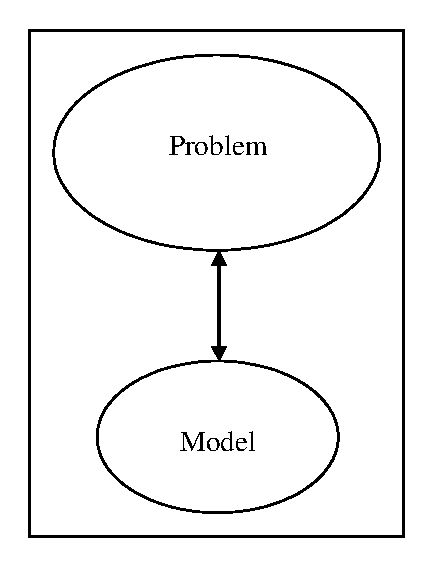
\includegraphics[scale=0.50]{IIDLE/mapping-cells-global}
	\end{minipage}}%
	\hfill
	\subfloat[Independent Sub-Models.]{
	\label{fig:mapping:cells:model:sub} %% label
	\begin{minipage}[t]{0.30\textwidth}
		\centering \includegraphics[scale=0.50]{IIDLE/mapping-cells-submodel}
	\end{minipage}}%
	\hfill
		\subfloat[Dependent Partial-Models.]{
	\label{fig:mapping:cells:model:partial} %% label 
	\begin{minipage}[t]{0.30\textwidth}
		\centering 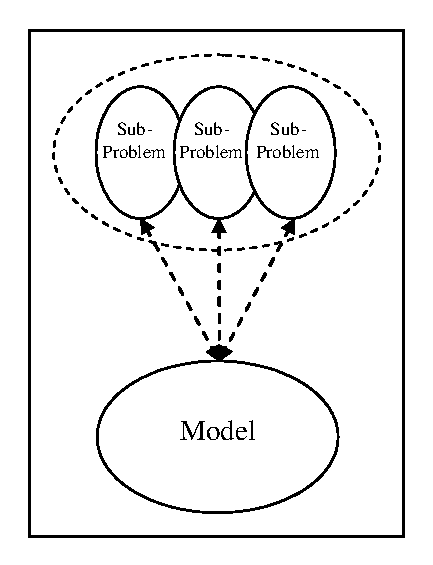
\includegraphics[scale=0.50]{IIDLE/mapping-cells-partialmodel}
	\end{minipage}}\\
	% end
	\caption{Depiction of the cellular algorithm approach to inductive learning with holistic, sub-, and partial-models of a given problem.}
	\label{fig:mapping:cells:models} %% label for entire figure
\end{figure}

% colour space
The three inductive modelling types may be related to the Antigen Colour Space Problems (ACSP) investigated in Chapter \ref{chap:cells}. The exposure of a single antigen ($N_{antigen}=1$) to the system may be considered an independent model, whereas the multiple antigen ($N_{antigen}=N$) and explicit aggregation of solutions may be considered the modelling of multiple independent sub-problems. Importantly, given that the ACSP definition did explicitly partition the antigenic set, although did not define the ordering of the exposure of patterns to the system, the ($N_{antigen}=N$) problem case may be considered a holistic problem with unknown sub-problems and therefore given this unknown must be modelled using partial-dependent sub-models (problem-side aggregation of responses). If the ordering of antigenic exposures was known to the system, then explicit sub-repertoires could be defined and specialised for each pattern (system-side aggregation of responses). Finally, the modelling of colour space patterns using colour components (in the case of DCCSA) may be considered the modelling of the ACSP using independent cellular components (one-cell equals one-component), although the modelling of sub-symbolic determinants (such as partial strings) would have provided an example of dependent partial modelling of single antigen. 


%
% Feature Summary
%
\subsubsection{Feature Summary}
This section summarises the important descriptive features of Cellular Clonal Selection Algorithms, and projects their features onto general features of problems to which this class of algorithm may be suitable for application.

%
% Salient System Features 
%
\paragraph{Salient System Features}
The following provides a list of the five features identified as being distinctive in characterising the general class of Cellular Clonal Selection Algorithms. 

\begin{itemize}
	\item \emph{Selectionist Adaptation}: Relative improvement of the system's decision making capability in the context of a problem via a process of selection and decent with modification to iteratively acquire and refine acquired information.
	\item \emph{Inductive Learning}: Information is acquired and generalised from discrete and specific examples provided by the problem.
	\item \emph{Stochastic Process}: The interaction with the problem and the resultant adaptation have an inherent element of randomness that promotes approximation of acquired information, general robustness of the system to noise, and flexibility of the system to unexpected events. 
	\item \emph{Population-based}: Maintenance of a diverse although clustered set (inherent redundancy) of pre-committed structures by the system, each of which may interact with the problem potentially in a concurrent manner (inherent parallelism).	
	\item \emph{Pattern Recognition}: The acquisition of information and overt decision making are coupled and triggered via a pattern recognition mechanism and response to information from the problem.
\end{itemize}

%
% Projected Problem Features
%
\paragraph{Projected Problem Features}
The following provides a projection of the characterising features of Cellular Clonal Selection Algorithms onto general problem features to which such algorithms are expected to be suitable.

\begin{itemize}
	\item \emph{Discrete}: The problem is comprised of discrete packets information to which it is in the systems best interest to respond.	
	\item \emph{Online}: Continuous decision making and improvement are desired given the variable and potential dynamic or adversarial manner in which information is made available to the system.	
	\item \emph{Unknowns}: Many of the parameters and/or constraints of the problem are known, although important elements regarding the information content and/or ordering of the exposure of information remain unknown to the system.	
	\item \emph{Noise}: The information signal may be disrupted, intermittent, and/or noisy requiring a level of robustness of interpretation.	
	\item \emph{Regularities}: Problem information contains regularities or patterns that must be exploited for effective progress to be made by a system.
\end{itemize}


%
% Tissue Algorithms as Data Fusion
%
\subsection{Tissue Algorithms as Data Fusion}
This section reviews the general properties of tissue algorithms as an adaptive data fusion approach, and considers the approach that such algorithms are useful for the inductive modelling using different perspectives of a given problem. Finally, the general tissue algorithm features are listed, and projected onto suitable general problem features.

%
% Tissue Algorithm Overview
%
\subsubsection{Tissue Algorithms Overview}
% generally
Tissue algorithms are \emph{explicitly decentralised}, with each tissue providing an adaptive process making local decisions and improvements, the effects of which are \emph{implicitly integrated} into holistic understanding of the information environment. The induction of the information content and anticipated exposure is extended across each point of exposure providing a \emph{spatial acquisition and anticipation}, that trades-off concerns of localisation and dissemination. The tissue architecture is pre-determined, with \emph{tightly coupled} and \emph{fixed neighbourhood relationships} between tissues. Tissues themselves are not redundant, nor flexible in their topology (additions, modifications, deletions), although each tissues cellular information content is redundant, allowing general or specific loss of random sets of cells. The information composition across tissues is generally heterogeneous given the specialisation of each tissue (given an asymmetric information exposure pattern), although the general capability at any tissue in the system is equivalent (\emph{heterogeneous composition, homogeneous capability}). This equivalence in capability is provided by the continuous dissemination (high frequency, generally low amplitude) of the underlying system information, and the localised as well as opportunistic way in which such information is exploited.
% data fusion
The general method is called \emph{multisensor data fusion} (information fusion or distributed sensing) whereby the modularity of information acquisition is exploited and combined for holistic application providing an improved model over that of a series of independent models \cite{Hall2004}.  The modularity may be imposed requiring explicit decomposition or partitioning of an information environment using prior information. Alternatively, the modularity of the information and its integration with the system may be an inherent feature of the environment. In this latter case, the interaction with the environment governed by the tissue exposure regime may or may not be known, making information acquisition and application \emph{opportunistic}. Integration is achieved by the continuous recirculation and mixing of acquired information, suggesting that the application of the integrated information may also be piece-wise or modular like the acquisition of the information (so-called piecewise acquisition and application from the system perspective, or exposure and expectation from the environment perspective).

%
% Inductive Model Generation
%
\subsubsection{Inductive Model Generation}
% models
The tissue algorithms may be considered in the context of the three generative inductive models, specifically independent models and sub-models, and dependent partial models.
% general 
Figure~\ref{fig:mapping:tissue:models} depicts the general relationship between the tissue algorithms and the three modelling types in the context of problem instances that support such modelling. The architecture of tissue algorithms forces an an explicit partitioning of a given problem information space whether such partitioning exists or not. 
% colour space
The partitioning of the Infection Antigenic Exposure Problem (IAEP) via the Tissue Exposure Regimes provides a basis for considering the suitability of the tissue model against each modelling type (Chapter \ref{chap:tissues}). In the case of a holistic modelling, one may consider a symmetric or point exposure regime in which case the persistent unbiased recirculation generally provides a disruptive influence to such modelling. Similarly, one may consider an asymmetric exposure regime representative of an explicit decomposition of the problem, where persistent unbiased recirculation has the same disruptive effects. 
% not suitable
Specifically, the results suggest, that although the tissue algorithms can construct such inductive models (innate capability), \emph{tissue algorithms may not be suitable for constructing holistic or sub-models unless there is an expectation that dissemination will be beneficial}, for example in the problem definition, or if the intra-tissue CCSA is capable of exploiting such information\footnote{This latter example was demonstrated to not be the case for in the use of RCCSA as an intra-tissue algorithm.}. This finding is further supported by analogous findings from related approaches in Section~\ref{subsec:iidle:function:optimization:applicability} and Section~\ref{subsec:iidle:function:approximation:applicability}.
%
% relates to architecture things, for example ATER - good for specialised entry points (food, nostril, etc)
% highlights, I should relate te exposure regimes to things in the physiology of such systems
%

% plots
\begin{figure}[htp]
	\subfloat[Independent Models.]{
	\label{fig:mapping:tissues:model:global} %% label 
	\begin{minipage}[t]{0.30\textwidth}
		\centering 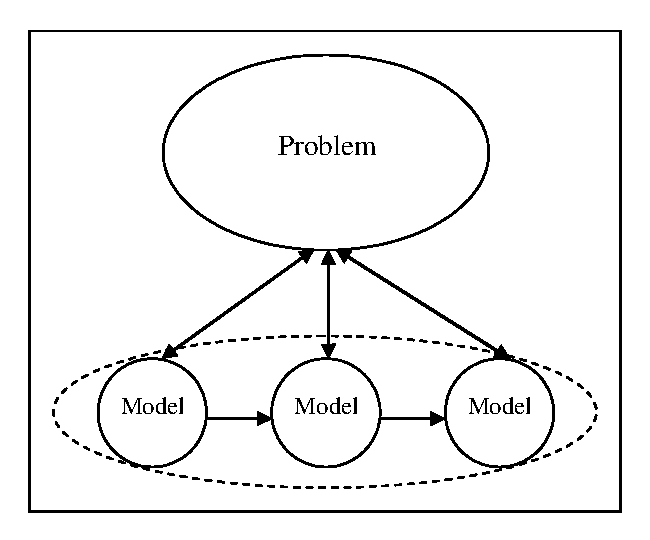
\includegraphics[scale=0.45]{IIDLE/mapping-tissues-global}
	\end{minipage}}%
	\hfill
	\subfloat[Independent Sub-Models.]{
	\label{fig:mapping:tissues:model:sub} %% label 
	\begin{minipage}[t]{0.30\textwidth}
		\centering 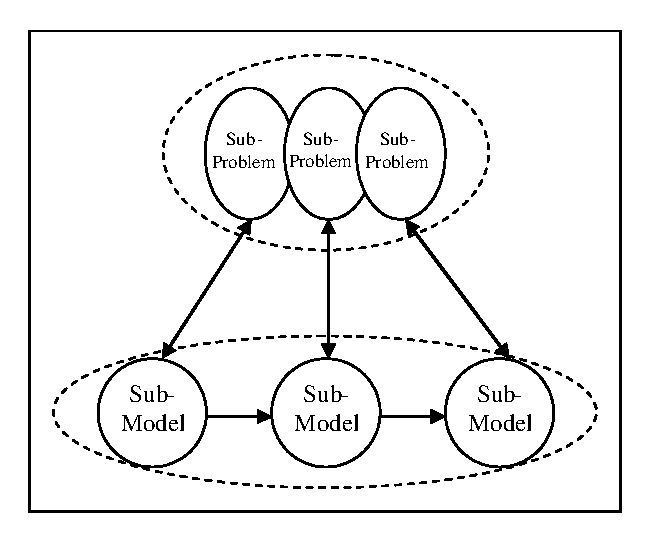
\includegraphics[scale=0.45]{IIDLE/mapping-tissues-submodel}
	\end{minipage}}%
	\hfill
		\subfloat[Dependent Partial-Models.]{
	\label{fig:mapping:tissues:model:partial} %% label 
	\begin{minipage}[t]{0.30\textwidth}
		\centering 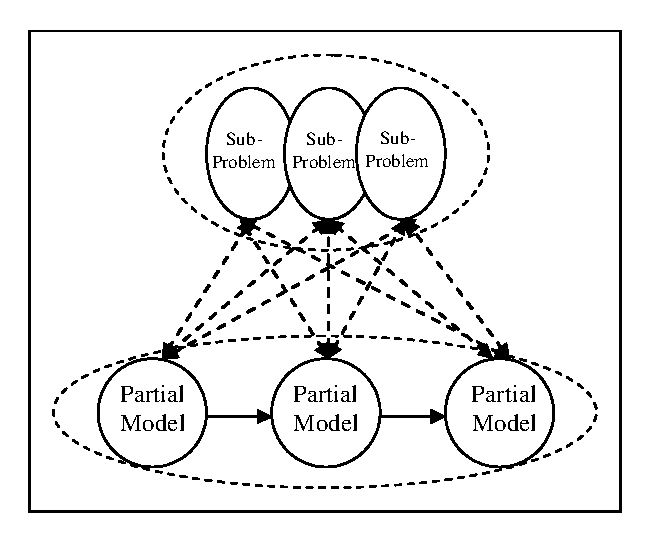
\includegraphics[scale=0.45]{IIDLE/mapping-tissues-partialmodel}
	\end{minipage}}\\
	% end
	\caption{Depiction of the tissue algorithm approach to inductive learning with holistic, sub-, and partial-models of a given problem.}
	\label{fig:mapping:tissue:models} %% label for entire figure
\end{figure}

% suitable
Importantly, the functional decomposition was not included in the IAEP definition, therefore, the tissue algorithms may be considered to have constructed partial models for the unknown sub-problems in the problem definition (TER's). As such, the aggregation of results for a specific TCSA across the TER's provides a general indication of algorithm capability. The aggregation of results clearly highlight that MTCSA is more suitable for per-exposure responses, and that the \emph{recirculation algorithms may be more suitable for holistic solution aggregation at any given single tissue under an unknown exposure regime}, likely at any given time under such a regime. More specifically, this suggests the suitability of recirculation tissue approaches are with the redundancy of acquired information to data loss and impromptu localised solution aggregation.
% suggests it can support data loss, impromptu solution aggregation
Beyond this general suitability, the results also suggest the specific suitability of recirculation methods under a random exposure regime compared to the non-recirculation approach. Although the exploratory results from Chapter \ref{chap:tissues} are not conclusive, they suggest strong constraints on the suitability of applicability of recirculation-based Tissue Clonal Selection Algorithms.


%
% Feature Summary
%
\subsubsection{Feature Summary}
This section summarise the important descriptive features of Tissue Clonal Selection Algorithms, and projects the features onto general features of problems to which this class of algorithm may be suitable for application.

%
% Salient System Features 
%
\paragraph{Salient System Features}
The following provides a list of the five features identified as being distinctive in characterising the general class of (recirculation-based) Tissue Clonal Selection Algorithms. 

\begin{itemize}
	\item \emph{Distributed Model}: The population-based model is distributed across a series of discrete and communicating sub-populations. 
	\item \emph{Decentralised Adaptation}: Acquisition of information and decision making occurs locally at each distributed point of the system providing a natural mapping for problems that can be functionally or logically decomposed.
	\item \emph{Tight Coupling}: Sub-populations are organised in a spatial topology with fixed neighbourhood relationships that generally communicate a low amplitude of information with a high frequency. 
	\item \emph{Data Fusion}: Information acquired in localised regions of the structure is disseminated and made available across the system, providing an integrated although distributed holistic model.
	\item \emph{Opportunistic}: The general availability of acquired information and decision making capability facilitates the opportunistic exploitation of variably accessible problem information or information processing capability.
\end{itemize}

%
% Projected Problem Features
%
\paragraph{Projected Problem Features}
The following provides a projection of the characterising features of Tissue Clonal Selection Algorithms onto general problem features to which such algorithms are expected to be suitable.

\begin{itemize}		
	\item \emph{Discrete Decomposition}: In addition to facilitating discrete interaction with the system, the problem should be able to be functionally or logically decomposed into sub- or partial problems which are naturally or explicitly partitioned across points of contact with the system.
	\item \emph{Online}: It is desirable for a holistic system to achieve continuous improvement against the problem, although less sensitive with regard to behaviour across specific spatial interactions.
	\item \emph{Spatial-Temporal Regularities}: The notions of noisy information signals and regularities extend beyond sub-problems, and extend across the spatially discrete interactions with the system (notions of Tissue Exposure Regimes).		
	\item \emph{On Demand}: Information and/or decision making capability acquired by the system holistically is required at a single given point of the system in an as needed manner (impromptu and point-wise solution aggregation).
	\item \emph{Hazardous Environment}: Addressing the problem requires some level of system robustness with regard to the loss, corruption, or failure of general (random sample from all tissues) or specifically-localised (content of random tissue or information in transit) sub-sets of information acquired by the system.
\end{itemize}


%
% Host Algorithms as Mixtures of Experts
%
\subsection{Host Algorithms as Mixtures of Experts}
This section reviews the general properties of host algorithms as an adaptive mixture of experts approach, and considers the application of such algorithms for the use in inductive modelling, expliting different perspectives of a given problem. Finally, the general host  algorithm features are listed, and projected onto suitable general problem features.

%
% Tissue Algorithm Overview
%
\subsubsection{Host Algorithms Overview}
% generally
Like tissue algorithms, host algorithms are comprised of a set of \emph{decentralised processes making localised decisions}, that in aggregation represent the systems information composition and general capability. Unlike the tissue paradigm, hosts are loosely coupled, without fixed neighbourhood relationships. The localised adaptive processes are \emph{quasi-independent} and their interactions are impromptu, opportunistic, and generally peer-to-peer. Their quasi-independence is reflected in their perspectives of the information environment, where interactions do not promote an integration of perspectives, rather are \emph{low-bandwidth dissemination of information} (low frequency, generally high amplitude of cells) from which, in aggregation the population is expected to benefit. As such information dissemination is selective and organised although impromptu given the generally unstructured nature of the population of hosts.
% mixture of experts
The general method is called \emph{mixture of experts} (ensemble methods) where systems exploit the modularity of the perspectives of the information environment by specialising in separate although potentially overlapping perspectives \cite{Opitz1999, Polikar2006}. As with the data fusion perspective of the tissue paradigm, the modularity of the environment may be imposed through explicit decomposition or partitioning, or may be an inherent feature of the environment.
% restarts
Each host generates a model of its perspective of the information environment through the cellular and tissues process of induction via adaptation. The generational host algorithms relate to the general method called \emph{multiple restarts} (iterative restarts or multiple runs) as this generative process is periodically reinitialised for a different although potentially biased set of starting conditions that influence the inductive model generation process \cite{Hu1994, Cantu-Paz2003}.

%
% Inductive Model Generation
%
\subsubsection{Inductive Model Generation}
% models
The host algorithms may be considered in the context of the three generative inductive models, specifically independent models and sub-models, and dependent partial models.
% general 
Figure~\ref{fig:mapping:host:models} provides a depiction of general host algorithms with regard to the three inductive model types. The figures show the explicit partitioning of the model, as was the case with the tissue algorithms.
% colour space
Also as with the tissue algorithms, spatial exposures regimes were the focus of the capabilities of the host algorithms embodied in the Habitat Antigenic Exposure Problem (HAEP). Model generation can be considered with regard to the population-based and generation-based approaches separately. 
% population models
In the case of a holistic and sub-model generation the non-interaction MP-HCSA demonstrated its suitability with regard to exposure-wise aggregation of results (system error), and its lack of suitability for impromptu point-wise aggregation of results in the same manner as the MTCSA. Interestingly, both the Random-Pairing Pathogen Transmission HCSA and the Small Sample SI-HCAS demonstrated a trend of decreased point-wise aggregation error and in the latter case system error. This highlights the \emph{suitability of population-based HCSA with small unstructured dissemination of acquired information or triggers not only for holistic (SHER) and sub-models (AHER), but also for partial models (across unknown HER's)}, in particular, SI-HCSA-SS was competitive with MP-HCSA under the AHER and SHER exposure regimes.

% plots
\begin{figure}[htp]
	\subfloat[Independent Models.]{
	\label{fig:mapping:hosts:model:global} %% label 
	\begin{minipage}[t]{0.30\textwidth}
		\centering 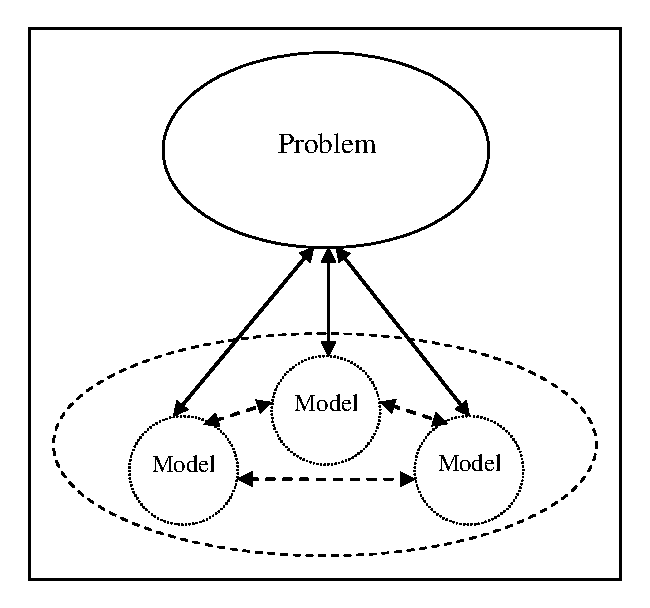
\includegraphics[scale=0.45]{IIDLE/mapping-hosts-global}
	\end{minipage}}%
	\hfill
	\subfloat[Independent Sub-Models.]{
	\label{fig:mapping:hosts:model:sub} %% label 
	\begin{minipage}[t]{0.30\textwidth}
		\centering 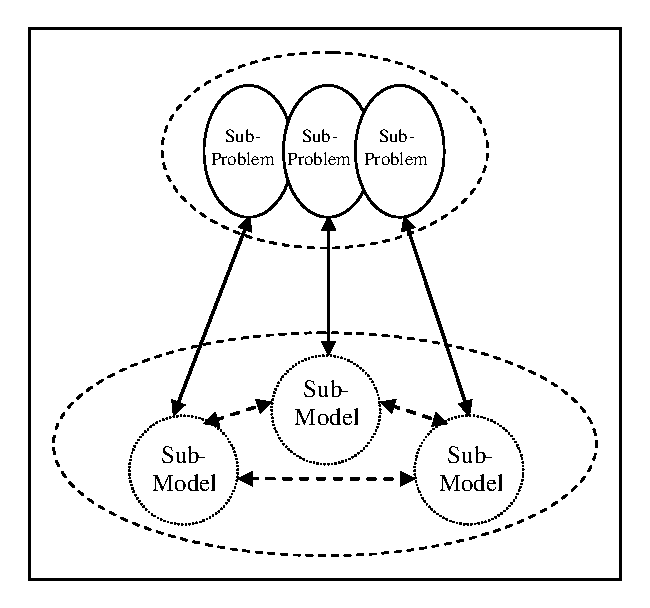
\includegraphics[scale=0.45]{IIDLE/mapping-hosts-submodel}
	\end{minipage}}%
	\hfill
		\subfloat[Dependent Partial-Models.]{
	\label{fig:mapping:hosts:model:partial} %% label 
	\begin{minipage}[t]{0.30\textwidth}
		\centering 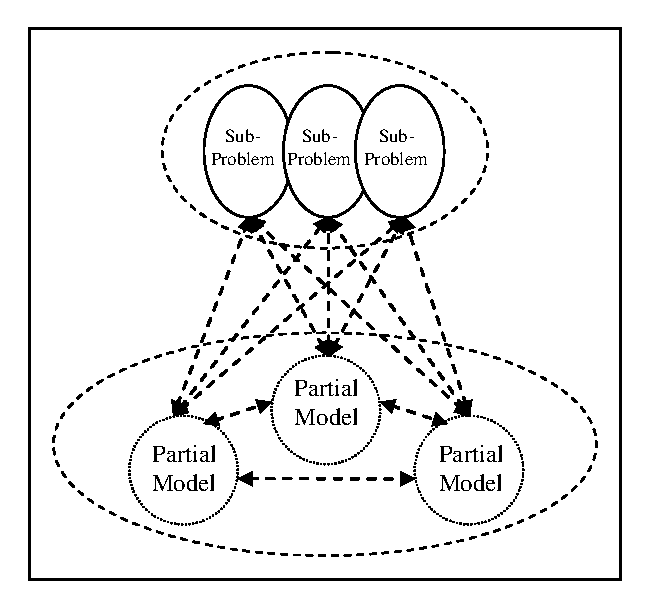
\includegraphics[scale=0.45]{IIDLE/mapping-hosts-partialmodel}
	\end{minipage}}\\
	% end
	\caption{Depiction of the host algorithm approach to inductive learning with holistic, sub-, and partial-models of a given problem.}
	\label{fig:mapping:host:models} %% label for entire figure
\end{figure}

% generational models
The generational approach of host populations provides capability for restarting the model generation process that may remove specific training biases by using varied starting conditions. Further, the adaptation of the model generation process itself in the EI-HCSA provides capability for tuning the process toward improved resultant models. Although capable, neither approach was demonstrated suitable for such application from the results of the limited exploratory experimentation, likely given the specifics of the configurations used.

%
% Feature Summary
%
\subsubsection{Feature Summary}
This section summarise the important descriptive features of Host Clonal Selection Algorithms, and projects their features onto general problem features to which this class of algorithm may be suitable for application.

%
% Salient System Features 
%
\paragraph{Salient System Features}
The following provides a list of the five features identified as being distinctive in characterising the general class of Host Clonal Selection Algorithms. 

\begin{itemize}
	\item \emph{Distributed Model}: The generation, storage and maintenance of the inductive model is distributed across a set of discrete and communicating sub-systems, where the acquisition of information and decision making is decentralised across the discrete contacts with the problem promoting a natural mapping for partitioned or partitionable problems.	
	\item \emph{Loose Coupling}: Sub-systems are not organised into any explicit spatial topology, therefore neighbourhood interactions are impromptu, generally involving a small number of sub-systems communicating a moderate amplitude of information with a low frequency.	
	\item \emph{Mixture of Experts}: Sub-systems become specialists in potentially overlapping partitions of the problem space, from which infrequent intra-population communication benefits the quasi-independent partial and/or sub-models.	
	\item \emph{Multiple Restarts}: The generational concerns of the model provide an iterative restart mechanism providing multiple model generational trials that may be selectively biased.
	\item \emph{Adaptation of Process}: The evolutionary generational concerns of the model provide an iterative adaptation mechanism for improving the model generation process with regard to a specific problem `environment'.	
\end{itemize}

%
% Projected Problem Features
%
\paragraph{Projected Problem Features}
The following provides a projection of the characterising features of Host Clonal Selection Algorithms onto general problem features to which such algorithms are expected to be suitable.

\begin{itemize}
	\item \emph{Discrete Partitions}: The problem must facilitate discrete interaction with the sub-systems, and likely be comprised of or partitioned into multiple sub- or partial problems to which each sub-system may specialise. 
	\item \emph{Online Improvement}: It is desirable for the system to promote continuous iterative improvement holistically (across sub-systems) likely in response to varying information or exposure patterns, although there is less of a concern for per sub-system improvement.
	\item \emph{On Demand}: Access to the acquired information and/or acquired decision making capability from across all sub-systems may be required holistically at a single point of interaction with the problem in an impromptu manner.
	\item \emph{Unclear Constraints}: The constraints of inductive model generation may be unknown on unclear requiring multiple trials for generating models, and/or a meta-process to improve the model generation process.
	\item \emph{Hazardous Environment}: The computational environment in which the sub-systems must operate to address the problem may be hazardous, resulting in the in the loss of whole sub-systems and/or sub-sets of acquired information.	
\end{itemize}


% 
% Function Optimisation
%
\section{Function Optimisation}
\label{sec:iidle:function:optimization}
% relation to ai and ci
Real-world optimisation problems and generalisations thereof can be drawn from most fields of science, engineering, and information technology (for a sample see \cite{Ali1997, Toern1999}). Importantly, optimisation problems have had a long tradition in the fields of Artificial Intelligence and Computational Intelligence in motivating basic research into new problem solving techniques, and for investigating and verifying systemic behaviour against benchmark problem instances.
% this section
This section considers the \emph{Function Optimisation Formalism} and related specialisations as a general motivating problem for demonstrating the suitability of the applicability of clonal selection algorithms from across the hierarchical framework.
% specifically
This is achieved firstly with a review of the problem formalism, nomenclature, and related sub-fields. Selected Artificial and Computational Intelligence research is reviewed that demonstrate feature overlap with concerns from at least one of the three clonal selection paradigms, highlighting relevant problem features that such algorithms may exploit. Finally, the Cellular, Tissue, and Host Clonal Sselection Paradigms are mapped onto general cases of Function Optimisation problems to which they are suited.

%
% Function Optimisation Overview
%
\subsection{Function Optimisation Overview}
\label{subsec:iidle:function:optimization:overview}

%
% Problem Definition
%
\subsubsection{Problem Description}
% definition
Optimisation (in the mathematical sense), is defined as the search for a combination of parameters commonly referred to as \emph{decision variables} ($x = \left\{x_1, x_2, x_3, \ldots x_n\right\}$) which minimise or maximise some ordinal quantity ($c$) (typically a scalar  called a score or cost) assigned by an \emph{objective function} or \emph{cost function} ($f$), under a set of constraints ($g = \left\{g_1, g_2, g_3, \ldots g_n\right\}$). For example, a general minimisation case would be as follows: $f(x\prime) \leq f(x), \forall x_i \in x$. Constraints may provide boundaries on decision variables (for example in a real-value hypercube $\Re^n$), or may generally define regions of feasibility and infeasibility in the decision variable space or cost space. In applied mathematics the field may be referred to as \emph{Mathematical Programming}. More generally the field may be referred to as \emph{Global} or \emph{Function Optimisation} given the focus on the objective function (for more general information on optimisation, see \cite{Horst2000, Project1995, Boyd2004}). 

%
% Sub-fields
%
\subsubsection{Sub-Fields of Study}
% general taxonomy
The study of optimisation is comprised of many specialised sub-fields, generally based on an overlapping taxonomy that focuses on the principle concerns in the general formalism. 
% general fields
For example, with regard to the decision variables, one may consider univariate and multivariate optimisation problems. The type of decision variables promotes the specialities for continuous, discrete, and permutations of variables. Dependencies between decision variables under a cost function defines the fields of Linear Programming, Quadratic Programming, and Nonlinear Programming. A large class of optimisation problems can be reduced to discrete sets, which are considered in the field of Combinatorial Optimisation, to which many theoretical properties are known, most importantly that many interesting and relevant problems cannot be solved by an approach with polynomial time complexity (so-called NP-complete, for example see \cite{Papadimitriou1998}).

% need for more complex models
The topography of the response surface for the decision variables under the cost function may be convex, which is an important class of functions to which many important theoretical findings have been made, not limited to the fact that location of the local optimal configuration also means the global optimal configuration of decisional variables has been located \cite{Boyd2004}. Many interesting and real-world optimisation problems produce cost surfaces that are non-convex or so called multi-modal\footnote{Taken from statistics referring to the centres of mass in distributions, although in optimisation it refers to `regions of interest' in the search space, in particular valleys in minimisation, and peaks in maximisation cost surfaces.} (rather than uni-modal) suggesting that there are multiple peaks and valleys. Further, many real-world optimisation problems with continuous decision variables cannot be differentiated given their complexity or limited information availability meaning that derivative-based gradient decent methods that are well understood are not applicable, requiring the use of so-called `direct search' (sample or pattern-based) methods \cite{Lewis2000}. Further, real-world objective function evaluation may be noisy, non-continuous, and dynamic, and the constraints of real-world problem solving may require a viable or approximate solution in limited time or resources, motivating the need for inductive model-generation based approaches.

%
% Selected Examples
%
\subsubsection{Selected Examples}
This section reviews a select set of approaches toward addressing optimisation problems from the field of Artificial and Computational Intelligence to both provide general insight into the state of the interaction between stochastic algorithms and the field of optimisation, and to provide a context for relating the clonal selection algorithms to optimisation problems by analogy. This section draws heavily from the field of Evolutionary Computation, Swarm Intelligence, and related Computational Intelligence sub-fields (see Section~\ref{sec:cs:related}).

\begin{itemize}
	
	\item \emph{Global and Local Optimisation}: Global Optimisation refers to seeking a globally optimal structure or approximation thereof, typically in an unconstrained $n$-dimensional real valued space. Global is differentiated from Local Optimisation in that the latter focuses on locating an optimal structure within a constrained region of the decision variable search space, such as a single peak or valley (basin of attraction). In AI and CI literature, global optimisation problems refers to the class of optimisation problems that generally cannot be addressed through more conventional approaches such as gradient decent methods (that require derivatives), and pattern search (that can get `stuck' in local optima and/or may never converge) \cite{Price1977, Toern1999}. Such problems are typically addressed through a directed search strategy with stochastic elements, typically involving a population-based model in the case of global search (for example a GA, see Section~\ref{subsec:cs:related:ec}), and a mutation hill climbing-based model for local search (see Section~\ref{subsec:cs:related:hillclimbing}). The general strategy involves sampling broadly initially, and converging on those areas of the search space that are most likely to payoff toward the end of the search. It is common to apply a local search method to the solutions of a global search procedure as an refinement strategy.
	
	\item \emph{Parallel Optimisation}: A natural first step in addressing difficult (large and rugged cost landscapes) is to exploit parallel and distributed hardware, to get an improved result in the same amount of time, or the same result in less time, or both \cite{Crainic2005}. Towards unifying the myriad of approaches and hardware configurations, a general consensus and taxonomy has been defined by the Parallel Evolutionary Algorithms (PEA) and Parallel Metaheuristics fields that considers the ratio of \emph{communication} to \emph{computation} called \emph{granularity} \cite{Cantu-Paz2000, Alba2005a}. This taxonomy is presented concisely by Alba and Tomassini as a plot or trade-off of three concerns: (1) the number of sub-populations (models or parallel strategies working on the problem), (2) the coupling between the sub-populations (frequency and amplitude of communication), and (3) the size of the sub-populations (size or extent of the sub-models) \cite{Alba2002}. Two important and relevant findings from the narrower field of Parallel Evolutionary Algorithms include (1) that tightly coupled (frequent migration) between coarse-grained models typically results in worse performance than a non-distributed approach \cite{Alba2000}, and (2) that loose coupling (infrequent migration) between coarse-grained models has been consistently shown to provide a super-linear increase in performance \cite{Alba2002a, Belding1995, Cantu-Paz2000}.
	
	\item \emph{Cooperative Search}: This is a more general approach that considers the use of multiple models that work together to address a difficult optimisation problems. Durfee, et~al. consider so-called \emph{Cooperative Distributed Problem Solving (CDPS)} in which a network of loosely coupled solvers are employed to address complex distributed problems. Specifically, such systems are desirable to match the processing capabilities of the solver with regard to the attributes of the problem. For example, a given problem may have spatially distributed, functionally distributed, or temporally distributed sub-problems to which a centralised and monolithic system may not be suitable. Lesser considers CDPS and proposes such models perform \emph{distributed search} on dependent or independent and potentially overlapping sub-problems as a motivating perspective for conducting research into Distributed Artificial Intelligence (DAI)\footnote{This perspective provided the basis for what became the field of Multi-Agent Systems (MAS).} \cite{Lesser1990}. Lesser points out that in real world applications, it is hard to get a optimal mapping between the allocated resources to the needs or availability of information for a given problem, suggesting that such problems may be caused by a mismatch in processing times and/or number of sub-problems, interdependencies between sub-problems, and local experts whose expertise cannot be effectively communicated. For a more detail on the relationships between parallel and cooperative search, El-Abd and Kamel provide a rigorous taxonomy \cite{El-Abd2005}.
	
	\item \emph{Hybrid Search}: Hybrid Search is a perspective on optimisation that focuses on the use of multiple and likely different approaches either sequentially (as in the canonical global and local search case), or in parallel (such as in Cooperative Search). For example in this latter case, it is common in the field of PEA to encourage different levels of exploration and and exploitation across island populations by varying the operators or operator configurations used \cite{Tanese1989, Adamidis1996}. Talbi proposed a detailed 4-level taxonomy of Hybrid Metaheuristics that encompassed concerns of parallel and cooperating approaches \cite{Talbi2001}. The taxonomy encompasses parallel and cooperative considerations for optimisation and focuses on the discriminating features in the lowest level such as heterogeneity, and specialisation of approaches.
	
	\item \emph{Functional Decomposition}: Three examples of a functional decomposition of optimisation include (1) multiple objectives, (2) multiple constraints, and (3) partitions of the decision variable search space. Multi-Objective Optimisation (MOO) is a sub-field that is concerned with the optimisation of decision variables under a set of objective functions. A solution to a MOO conventionally involves locating and returning a set configurations under the objective functions called the optimal or non-dominated Pareto set of solutions \cite{Deb2001}. The complexity with MOO problems is in the typically unknown dependencies between decision variables across objectives, that in the case of conflicts, must be traded off (Purshouse and Fleming provide a taxonomy of such complexity \cite{Purshouse2003}). Constraint Satisfaction Problem's (CSP) involve the optimisation of decision variables under a set of constraints. The principle complexity in such problems is in locating structures that are feasible or violate the least number of constraints, potentially optimising such feasibility \cite{Tsang1993, Kumar1992}. Search Space Partitioning involves partitioning of the decision variable search space (for example see Multispace Search by Gu, et~al \cite{Du1997, Gu1997, Gu1994}). This is a critical consideration given that for equal-sized dimensions bounds on parameters, the increase in decision variables results in an exponential increase in the volume of the space to search.
			
	\item \emph{Availability Decomposition}: Optimisation problems may be partitioned by the concerns of temporal and spatial distribution of (1) information availability, and (2) computation availability. An interesting area of research regarding variable information availability for optimisation problems is called Interactive Evolutionary Computation, in which one or a collection of human operators dynamically interact with an optimisation process \cite{Takagi2001}. Example problem domains include but are not limited to computer graphics, industrial design, image processing, and drug design. There is an increasing demand to exploit clusters of heterogeneous workstations to complete large-scale distributed computation tasks like optimisation, typically in an opportunistic manner such as when individual machines are under utilised. The effect is that optimisation strategies, such as random partitioning of the search space (independent non-interacting processing) are required to take advantage of such environments for optimisation problems \cite{Schnekenburger1993, Liu2000}.
	
	\item \emph{Meta Optimisation}: One may optimisation at a level above that considered in previous sections. Specifically, (1) the iterative generation of an inductive model called multiple restart optimisation, and (2) the optimisation of the parameters of the process that generates an inductive model of an optimisation problem. Multiple or iterative restarts involves multiple independent algorithm executions from different (random) starting conditions. It is generally considered as an method for achieving an improved result in difficult optimisation problems in which a given strategy is deceived by local or false optima \cite{Muselli1997, Hu1994}, typically requiring a restart schedule \cite{Fukunaga1998}. A second and well studied form of meta optimisation involves the optimisation of the search process itself. Classical examples include the self-adaptation of mutation parameters (step sizes) in the Evolutionary Strategy \cite{Rechenberg1973, Schwefel1981} and Evolutionary Programming \cite{Fogel1966, Fogel1991} approaches. Smith and Fogarty provided a review of genetic algorithms with adaptive strategies providing a taxonomy in which the meta-adaptations are applied at one of three levels: (1) the population (adapting the overall sampling strategy), (2) the individual (adapting the creation of new samples in the decision variable space), and (3) components (modifying component contributions and/or individual step sizes as in ES and EP) \cite{Smith1997b}.
	
\end{itemize}


%
% Clonal Selection Applicability
%
\subsection{Clonal Selection Applicability}
\label{subsec:iidle:function:optimization:applicability}
This section considers the suitability of application of the clonal selection algorithms from across the Cellular, Tissue, and Host Paradigms to the general problem of Function Optimisation. Applicability is considered in the context of the algorithm features reviewed in Section~\ref{sec:iidle:suitability} against the selected examples reviewed in the previous section.

%
% Cellular Algorithms
%
\subsubsection{Cellular Algorithms}
\label{subsec:iidle:function:optimization:applicability:cells}
% mapping
A functional mapping of clonal selection onto the Function Optimisation formalism is as follows: \emph{cells} represent the decision variables (or a mapping thereof) that define a structure, \emph{antigen} is abstracted as the cost function and/or constraints imposed on the structure, the \emph{repertoire} represents a clonal set of cells specialised (converged) toward addressing the antigen in response to the \emph{affinity} assigned to structures by the cost function. 
% related CSA
This single-antigen mapping of clonal selection to the optimisation formalism was shown in in Section~\ref{subsec:cs:algorithms:taxonomy} to be the basis of the development and investigation of a variety of clonal selection algorithms not limited to CLONALG, BCA, and the IA family of algorithms where in each case a repertoire of cells was adapted to address a cost function. This mapping embodies the \emph{affinity maturation principle} reviewed in Section~\ref{subsec:cs:algorithms:principle} as a constrained clonal selection metaphor suitable for application to optimisation domains, specifically as a process directed toward the improvement of affinity (maturation) of cells in the context of an antigen.

% global and local optimisation
The general cellular algorithms (CCSA and RCCSA) are suited to global and local optimisation in the case where the objective function is mapped to an affinity interaction with a single antigen. One may consider the procedure a local search when a single cell is used ($N_{cells}=1$) and a multi-point global search procedure otherwise ($N_{cells}>1$). As such, the procedure is generally less sophisticated than a an Evolutionary or Swarm Intelligence approach, and belongs to the general class of directed random search, and (point and/or population-based) stochastic-based hill climbing and steady-state genetic algorithm without crossover (see Section~\ref{sec:cs:related}). 
% parallel
The point-wise basis to exposures across all cellular algorithms promotes considerations of parallelism within the repertoire, perhaps exemplified in the SCCSA which strongly resembles the so-called fine-grained parallisation of genetic algorithms for multi-processor hardware (such as diffuse and cellular genetic algorithms \cite{Pettey2000}).
% mediated and network
The mediated (ECCSA) and network (NCCSA) algorithms do not have clear analogies in the field of optimisation. Although these approaches are immature, further development may reveal their capability in learning complex inter-relationships between decision variables or other functional decompositions such as objectives, constraints, and regions in the search space.
% decomposition
Finally, one may consider the functional decompositions of optimisation problems and their mapping onto the foundational CCSA as either explicit sub-models or inferred partial models. The generality of these foundational approaches means that augmentation may be required to effectively manage explicit sub-problems such as MOO and CSP.
% summary
A summary of the suitability of application for the Cellular Clonal Selection Algorithms to Function Optimisation is provided in Table~\ref{tab:iidle:function:optimisation:cellular}.

\begin{table}[htp]
	\centering\small
		\begin{tabular}{lllll}
		\toprule
		\textbf{Algorithm} & \textbf{$N_{antigen}$} & \textbf{$N_{cells}$} & \textbf{Optimisation Strategy} & \textbf{Inductive Model} \\ 
		\toprule
		\emph{MCCSA} & 1 & 1 & Local Search & Holistic \\ 
		\emph{R/CCSA} & 1 & N & Global Search & Holistic/Partial \\ 
		\emph{R/CCSA} & N & N & Decomposition Search & Sub/Partial \\ 
		\emph{SCCSA}  & 1 & N & Parallel Global & Holistic/Partial  \\ 
		\emph{E/NCCSA}  & 1 & N & Decomposition Search & Partial \\
		\emph{E/NCCSA}  & N & N & Decomposition Search & Sub/Partial \\ 		
		\bottomrule
		\end{tabular}
	\caption{Summary of the projected applicability of Cellular Clonal Selection Algorithms to Function Optimisation Problems.}
	\label{tab:iidle:function:optimisation:cellular}
\end{table}

%
% Tissue Algorithms
%
\subsubsection{Tissue Algorithms}
\label{subsec:iidle:function:optimization:applicability:tissues}
% mapping
The functional mapping of tissue algorithms to Function Optimisation is as follows: \emph{tissues} are mapped onto different (logically or physically) global or local optimisation processes, \emph{recirculation} is mapped onto inter-process communication and any overheads associated with such communication (for example network latency and/or memory requirements), \emph{infections} may be mapped as single objective functions (single antigen), or comprised of a set of objective functions, constraints or other functional decompositions (multiple antigen). The \emph{tissue exposure regime} may be influenced by a pre-designed arrangement of tissues (architecture and network topology), or may represent the interaction of the system with a known or unknown functional or logical decomposition of a given problem.

% global and parallel
As considered in with cellular algorithms, a single tissue may be exploited for a global or local optimisation process. Multiple non-interacting tissues in the MTCSA may be considered parallel global search or parallel multiple restarts, whereas those algorithms that use recirculation (RTCSA, HTCSA, ITCSA) may be considered cooperative search parallel strategies.
% cooperative
Given the high-frequency nature of recirculation, the RTCSA fits in somewhere between coarse and fine-grained parallel algorithms, with a moderate population size, moderate number of tissues, and fixed (directed cyclic graph) topology. Importantly the reviewed findings from parallel EA's suggest that such a configuration may perform as well as or worse than a non-distributed model (single population) for global optimisation. 
% hybrid
Interestingly, such behaviour (strong competition and system-wide takeover) may be desirable if parallel tissues cooperate using hybrid global optimisation strategies. For example, variations on cellular algorithms (such as a global and local variation of a given CCSA), or the holistic replacement of CCSA with other similar approaches (such as evolutionary or swarm intelligence algorithms).
% decomposition
Finally, the tissue architecture provides a natural mapping for functional and availability decompositions of a given optimisation problem. For example, objectives, constraints, and search space partitions may be explicitly or randomly assigned to tissues of the algorithm, where recirculation promotes the cooperative concerns such as trade-off's between the sub-problems. The tissue architecture is suited to such problem descriptions, although this suitability may be further improved if the functional decomposition is motivated by an availability decomposition such as distributed information availability, event-driven (such as human interaction), or opportunistic allocation of computation time. 
% summary
Table~\ref{tab:iidle:function:optimisation:tissue} summarises the applicability of TCSA to Function Optimisation problems.

\begin{table}[htp]
	\centering\small
		\begin{tabular}{lllll}
		\toprule
		\textbf{Algorithm} & \textbf{$N_{infection}$} & \textbf{$N_{tissues}$} & \textbf{Optimisation Strategy} & \textbf{Inductive Model} \\ 
		\toprule
		\emph{MTCSA} & 1 & 1 & Global Search & Holistic \\ 
		\emph{MTCSA} & 1 & N & Parallel Global & Holistic \\ 
		\emph{MTCSA} & N & N & Parallel/Decomposition & Sub \\				
		\emph{R/H/ITCSA} & 1 & N & Cooperative/Hybrid & Holistic \\ 
		\emph{R/H/ITCSA} & N & N & Cooperative/Decomposition & Sub/Partial \\ 
		\bottomrule
		\end{tabular}
	\caption{Summary of the projected applicability of Tissue Clonal Selection Algorithms to Function Optimisation Problems.}
	\label{tab:iidle:function:optimisation:tissue}
\end{table}

%
% Host Algorithms
%
\subsubsection{Host Algorithms}
\label{subsec:iidle:function:optimization:applicability:hosts}
% mapping
The functional mapping of host algorithms to Function Optimisation is as follows: \emph{hosts} may map onto different (logically or functionally) global or local search processes ($N_{tissues}=1$ per $H$), or more interestingly onto groups of tightly-coupled clusters of global or local search processes ($N_{tissues}>1$ per $H$). Similarly, a habitat may be a single objective function ($N_{infection}=1$ per $B$), a set of objectives functions or constraints ($N_{infection}>1$ per $B$), or a set of holistic although different function optimisation problems ($N_{habitats}>1$). As with the mapping of the tissue paradigm, the complexity of the system-problem interaction is relegated to the (in this case host) exposure regime.

% global and parallel
Given the bracketing of tissues, one may consider the extent of capabilities of the tissue algorithm subsumed by a host or a population of hosts, as was the case between the tissue and cellular paradigms. As such, if we ignore (constrain to $N_{tissue}=1$) tissue cardinality, the MP-HCSA provides a set of independent global or local strategies. 
% cooperative parallel
The SI-HCSA may be exploited for cooperative parallel global optimisation, given their strong resemblance in configuration to parallel evolutionary algorithms. Specifically, the small to moderate number of hosts, moderate to large population sizes, and low frequency, low amplitude sharing of information (decrease in frequency compared to experimentation in Chapter \ref{chap:hosts}). Further, the sharing-based population host algorithms encourage an unstructured topology of impromptu host interactions, more akin to a P2P network topology than a master-server, star or other fixed topology commonly exploited by PEA's. 
% cooperate hybrid 
The cooperative relationship of SI-HCSA may also be exploited for hybrid optimisation, perhaps with an increased frequency of migration, as was the case in the exploratory experimentation. 
% cooperative on decompositions
As with tissue paradigm, the population-based host algorithms may exploit the natural modularity of optimisation problems in terms of their functional and information availability decompositions, although it is unclear whether the varied information sharing scheme of SI-HCSA would promote the sufficient level of integration of partial-models where required (dependent decompositions). Interesting, the THCSA, specifically the Pathogen and Vaccination variations promote the consideration of sharing the triggers of adaptation, in this case an explicitly partitioned or limited availability resources between nodes in the system. Where this mechanism is supported under the constraints of a specific problem. Such behaviour may promote an adaptive-self organisation of responsibility within the host population. 

\begin{table}[htp]
	\centering\small
		\begin{tabular}{lllll}
		\toprule
		\textbf{Algorithm} & \textbf{$N_{habitats}$} & \textbf{$N_{hosts}$} & \textbf{Optimisation Strategy} & \textbf{Inductive Model} \\ 
		\toprule
		\emph{MP-HCSA} & 1   & 1   & Global Search & Holistic \\ 
		\emph{MP-HCSA} & 1   & N   & Parallel Global & Holistic \\ 
		\emph{SI-HCSA} & 1   & N   & Parallel/Cooperative/Hybrid & Holistic \\ 		
		\emph{SI/THCSA}& N   & N   & Cooperative/Decomposition & Sub/Partial \\
		\emph{MG-HCSA} & 1/N & 1 & Sequential Iterative-Restarts & Holistic \\ 
		\emph{MG-HCSA} & 1 & 1/N & Parallel Iterative-Restarts & Holistic \\ 
		\emph{MI-HCSA} & 1 & 1/N & Multiple Restart/Meta & Holistic \\ 
		\emph{EI-HCSA} & 1 & N   & Meta-Optimisation & Holistic \\ 		
		\bottomrule
		\end{tabular}
	\caption{Summary of the projected applicability of Host Clonal Selection Algorithms to Function Optimisation Problems.}
	\label{tab:iidle:function:optimisation:hosts}
\end{table}

% restarts
The generational host algorithms provide an clear relationship to the meta-optimisation techniques. MG-HCSA with a single host provides a model for a sequential restart strategy, and a parallel restart strategy when configured with multiple hosts. 
% biased restarts
The MI-HCSA algorithm provides a restart strategy in which the initialisation of \naive\ systems is biased with acquired information. This strategy may be effective in environments where the availability is subject to frequent and unexpected change to seed new instances of host processes (such as in the exploitation of idle computation time in a network environment).
% meta
Finally, the suggestion of optimising the initial conditions in the EI-HCSA provides a link between the restart strategy in GHCSA and meta optimisation strategies that optimise the processes that operate on a given problem instance.
% applies to all
Importantly the meta optimisation strategies (restarts and optimisation of process) apply not only to all cellular and tissue approaches to which the hosts subsume, but also to the capabilities of the population-based host algorithms. 
% summary
Table~\ref{tab:iidle:function:optimisation:hosts} summarises the applicability of HCSA to function optimisation problems.

%
% Summary
%
\subsection{Summary}
\label{subsec:iidle:function:optimization:summary}
This section summarises the insight provided into the applicability of the clonal selection algorithms from across the three paradigms generally with regard to Function Optimisation, and specifically with regard to some specialisations of the problem and techniques for addressing the problem.

\begin{enumerate}
	% general
	\item \emph{General Suitability}
	\begin{enumerate}
		\item \emph{Mapping}: The mapping between the general clonal selection adaptive strategy and function optimisation is natural for the specific case of blindly adapting a clonal set for a single antigen.
		\item \emph{Systems}: Beyond the adaptive cellular level, the tissue and host paradigms provide a basis for decentralised and distributed optimisation, given a suitable problem mapping.
		\item \emph{Environments}: Global optimisation alone is insufficient to motivate application to tissue and host paradigms, requiring functional and availability decompositions of a given optimisation problem to provide an effective mapping of the problem to the antigenic exposure paradigm.
	\end{enumerate}
	
	% algorithms
	\item \emph{Algorithm Applicability}
	\begin{enumerate}
		\item \emph{Cellular}: R/CCSA are suitable for local and global optimisation tasks, potentially for functional decompositions of optimisation problems, and SCCSA is suitable for parallisation.
		\item \emph{Tissue}: MTCSA is suitable for parallel global optimisation, R/H/ITCSA are suitable for cooperative hybrid and potentially functional decomposition, and likely not suitable for cooperative global search.		
		\item \emph{Host}: MP-HCSA is suitable for parallel global search, SI-HCSA is suitable for parallel global search and likely cooperative hybrid and functional decomposition, THCSA variants are suitable for functional decompositions and potentially cooperative parallel optimisation. MG-HCSA is suitable for multiple restarts, MI-HCSA may be suitable for biased multiple restarts, and EI-HCSA suggests at meta optimisation with further extension.
	\end{enumerate}		
\end{enumerate}

%
% Function Approximation
%
\section{Function Approximation}
\label{sec:iidle:function:approximation}
% relation to ai and ci
The phrasing of real-world problems in the Function Approximation formalism are among the most computationally difficult considered in the broader field of Artificial Intelligence for reasons including: incomplete information, high-dimensionality, noise in the sample observations, and non-linearities in the target function.
% this section
This section considers the \emph{Function Approximation Formalism} and related specialisations as a general motivating problem for demonstrating the suitability of the applicability of clonal selection algorithms from across the hierarchical framework.
% specifically
Firstly the general problem is reviewed including standard nomenclature and a summary of sub- and related fields of study. Selected Artificial and Computational Intelligence research is reviewed that demonstrate feature overlap with concerns from at least one of the three clonal selection paradigms, highlighting relevant problem features that such algorithms may exploit. Finally, the Cellular, Tissue, and Host Clonal Selection Paradigms are mapped onto general cases of Function Approximation problems to which that are proposed to be well suited.


%
% Function Approximation Overview
%
\subsection{Function Approximation Overview}
\label{subsec:iidle:function:approximation:overview}

%
% Problem Definition
%
\subsubsection{Problem Description}
% definition
Function Approximation (in the mathematical sense) is an \emph{inductive problem} of finding a function ($f$) that approximates a target function ($g$), where typically the approximated function is selected based on a sample of observations ($x$, also referred to as the \emph{training set}) taken from the unknown target function.
% ML
In machine learning, the function approximation formalism is used to describe general problem types commonly referred to as \emph{pattern recognition}, such as classification, clustering, and curve fitting (so-called decision or discrimination function). Specifically, such general problem types are described in terms of approximating an unknown Probability Density Function (PDF), which underlies the relationships in the problem space, and represented to some degree in the sample data. This function approximation perspective of such problems is commonly referred to as \emph{statistical machine learning} and/or density estimation \cite{Fukunaga1990, Bishop1995}.

%
% Sub-Fields of Study
%
\subsubsection{Sub-Fields of Study}
% really hard
The function approximation formalism can be used to phrase some of the hardest problems faced by Computer Science, and Artificial Intelligence in particular such as natural language processing and computer vision. 
% general process
The general process focuses on (1) the collection and preparation of the observations from the target function, (2) the selection and/or preparation of a model of the target function, and (3) the application and ongoing refinement of the prepared model. 
% important problem types 
Some important problem-based sub-fields include: \emph{Feature Selection} where a feature is considered an aggregation of attributes, where only those features that have meaning in the context of the target function are necessary to the modelling process \cite{Kudo2000, Guyon2003}, \emph{Classification} where observations are inherently organised into labelled groups (classes) and a supervised process models an underlying discrimination function to classify unobserved samples, \emph{Clustering} where observations may be organised into inherent groups based on common features although the groups are unlabelled requiring a process to model an underlying discrimination function without corrective feedback, and \emph{Curve or Surface Fitting} where a model is prepared that provides a `best-fit' (or regression) for a set of observations that may be used for \emph{interpolation} over known observations and \emph{extrapolation} for observations outside what has been observed.

% optimisation
The field of Function Optimisation is related to Function Approximation, as many-sub-problems of Function Approximation may be defined as optimisation problems. As such many of the inductive modelling paradigms are differentiated based on the representation used and/or the optimisation process used to minimise error or maximise effectiveness on a given approximation problem. 
% problems
The difficulty of Function Approximation problems centre around (1) the nature of the unknown relationships between attributes and features, (2) the number (dimensionality) of of attributes and features, and (3) general concerns of noise in such relationships and the dynamic availability of samples from the target function.
% other problems
Additional difficulties include the incorporation of prior knowledge (such as imbalance in samples, incomplete information and the variable reliability of data), and problems of invariant features (such as transformation, translation, rotation, scaling and skewing of features).

%
% Selected Examples
%
\subsubsection{Selected Examples}
This section reviews a select set of approaches toward addressing Function Approximation problems from the field of Artificial and Computational Intelligence to both provide general insight into the state of the interaction between stochastic algorithms and the field, and to provide a context for relating the clonal selection algorithms to Function Approximation problems by analogy. The review draws heavily from the fields of artificial neural networks, specifically competitive learning, as well as related inductive machine learning fields such as instance based learning.

\begin{itemize}
	\item \emph{Vector Quantisation}: Vector Quantisation (VQ) refers to a method of approximating a target function using a set of exemplar (prototype or codebook) vectors. The exemplars represent a discrete sub-set of the problem, generally restricted to the features of interest using the natural representation of the observations in the problem space, typically an an unconstrained $n$-dimensional real valued space. The VQ method provides the advantages of a non-parametric model of a target function (like instance-based and lazy learning such as $k$NN, see Section~\ref{sec:cs:related}) using a symbolic representation that is meaningful in the domain (like tree-based approaches). The promotion of compression addresses the storage and retrieval concerns of $k$NN, although the selection of codebook vectors (the so-called quantisation problem) is a hard problem that is known to be NP-complete \cite{Garey1982}. More recently Kuncheva and Bezdek have worked towards unifying quantisation methods in the application to classification problems, referring to the approaches as Nearest Prototype Classifiers (NPC) and proposing a generalised nearest prototype classifier \cite{Kuncheva1998, Kuncheva1998a}.
	
	\item \emph{Parallelisation}: Instance-based approaches are inherently parallel given the generally discrete independent nature in which they are used, specifically in a case or per-query manner. As such, parallel hardware can be exploited in the preparation of the corpus of prototypes (parallel preparation), and more so in the application of the corpus given its read-only usage \cite{Aamodt1994, Nagendra1996, Plaza1997}. With regard to vector quantisation specifically, there is an industry centred around the design and development of VQ and WTA algorithms and circuits given their usage to compress digital audio and video data \cite{Nakada1999, Parhi1994}.
	
	\item \emph{Cooperative Methods}: Classical cooperative methods in the broader field of statistical machine learning are referred to as \emph{Ensemble Methods} \cite{Opitz1999, Polikar2006} or more recently \emph{Multiclassifier Systems} \cite{Ghosh2002}. \emph{Boosting} is based on the principle of combining a set of quasi-independent weak learners that collectively are as effective as a single strong learner \cite{Kearns1988, Schapire1992}. The seminal approach is called Adaptive Boosting (AdaBoost) that involves the preparation of a series of classifiers, where subsequent classifiers are prepared for the observations that are misclassified by the proceeding classifier models (creation of specialists) \cite{Schapire2003}. \emph{Bootstrap Aggregation} (bagging) involves partitioning the observations into $N$ randomly chosen subsets (with reselection), and training a different model on each \cite{Breiman1996}. Although robust to noisy datasets, the approach requires careful consideration as to the consensus mechanism between the independent models for decision making. \emph{Stacked Generalisation} (stacking) involves creating a sequence of models of generally different types arranged into a stack, where subsequently added models generalise the behaviour (success or failure) of the model before it with the intent of correcting erroneous decision making \cite{Wolpert1992, Ting1999}. 
	
	\item \emph{Functional Decomposition}: As demonstrated, it is common in ensemble methods to partition the dataset either explicitly or implicitly to improve the approximation of the underlying target function. A first important decomposition involves partitioning the problem space into sub-spaces based on the attributes, regular groups of attributes called features, and decision attributes such as class labels. A popular method for attribute-based partitioning is called the Random Subspace Method, involving the random partitioning of attributes to which specialised model is prepared for each (commonly used on tree-based approaches) \cite{Ho1998}. A related approach involves a hierarchical partitioning of attributes space into sub-vectors (sub-spaces) used to improve VQ-based compression \cite{Gersho1984}. Another important functional decomposition involves the partitioning of the set of observations. The are many ways in which observations may be divided, although common approaches include pre-processing using clustering techniques to divide the set into natural groups, additional statistical approaches that partition based on central tendency and outliers, and re-sampling methods that are required to reduce the volume of observations.
	
	\item \emph{Availability Decomposition}: The availability observations required to address function approximation in real-world problem domains motivate the current state of the art in Distributed Data Mining (DDM or so-called Collective Data Mining), Parallel Data Mining (PDM), and Distributed Knowledge Discovery in Database (DKDD) \cite{Kargupta2000}. The general information availability concerns include (1) the \emph{intractable volume of observations}, and (2) the \emph{spatial (geographical) and temporal distribution of information} \cite{Zaki1999}. It is common in many large real-world problems for it to be infeasible to centralise relevant observations for modelling, requiring scalable, load balancing, and incremental acquisition of information \cite{Skillicorn1999}. 
	
	\item \emph{Meta Approximation}: The so-called ensemble or multiple-classifier methods may be considered meta approximation approaches as they are not specific to a given modelling technique. As with function optimisation, meta-approaches may be divided into restart methods and meta-learning algorithms. The use of restart methods is a standard practice for connectionist approaches, and more generally in approaches that use random starting conditions and a gradient or local search method of refinement. The method provides an opportunity for over-coming local optima in the error-responds surface, when there is an unknown time remaining until convergence \cite{Magdon-ismail2000}, and can exploit parallel hardware to provide a speed advantage \cite{Blas2005}. Ensemble methods and variants are examples of meta approximation approaches, as well as the use of consensus classifiers (gate networks in mixtures of experts) to integrate and weight the decision making properties from ensembles. 
\end{itemize}


%
% Clonal Selection Applicability
%
\subsection{Clonal Selection Applicability}
\label{subsec:iidle:function:approximation:applicability}
This section considers the suitability of the application of the clonal selection algorithms from across the Cellular, Tissue, and Host Paradigms to the general problem of Function Approximation. Applicability is considered in the context of the algorithm features reviewed in Section~\ref{sec:iidle:suitability} against the selected examples reviewed in the previous section.

%
% Cellular Algorithms
%
\subsubsection{Cellular Algorithms}
\label{subsec:iidle:function:approximation:applicability:cells}
% mapping
A generalised mapping of clonal selection onto the Function Approximation formalism is as follows: \emph{cells} are exemplars (a.k.a. codebooks or prototypes) in the parameter space (or a mapping thereof) of the target function, \emph{antigen} are the sample of observations from the target function (therefore there are always $N$), the \emph{repertoire} represents an approximation of the target function adapted in the presence of the sample observations, and \emph{affinity} is calculated based on a distance metric between observations and exemplars. 
% related examples
As considered in the review of the state of clonal selection algorithm research (Section~\ref{subsec:cs:algorithms:taxonomy}), this was the perspective used in the development and application of AIRS to classification where exemplars quantised observations. This mapping was also used in the application of CLONALG to binary pattern recognition, and was the basis for the colour space problems investigated across the three clonal selection paradigms in this work. 
% related paradigms
As considered in paradigms related to the field of clonal selection algorithms in Section~\ref{sec:cs:related}, the algorithms competition-based approach to preparing the exemplars in response to the sample observations is related to the field of \emph{competitive learning}, whereas the interpretation of the resulting exemplars is related to the field of \emph{instance-based learning}, specifically $k$-Nearest Neighbours ($k$NN).

% colour space things
The cellular clonal selection algorithms provide a series of global optimisers suitable for vector quantisation, not unlike the use of EC, SA, and hill climbing for the same task. The general nature of VQ makes the cellular algorithms suitable for classification (Nearest Prototype Classifiers), clustering, and curve fitting. Given the competition-based interaction between exemplars and the unknown context-based relationships that such competition represents, it is reasonable to categorise the cellular clonal selection algorithms as the induction of partial-models. Although it is important to point out that it is the degree to which such relationships have meaning in the problem space that defines whether the exemplars may be considered partial (strongly related) or sub (weakly or unrelated) models of the broader function approximation problem. The iterative (per-exposure) competition based learning and decision making suggest at the general suitability of the approach to incremental and dynamic specialisations of the general problem. The spatial properties of SCCSA show similarities with projection-based clustering methods such as SOM and Neural Gas, although unlike those approaches SCCAS in its present form does not demonstrate the preservation of topological features. As with function optimisation, the role of ECCAS and NCCAS is not clear given the approaches immature although demonstrated similarities with sub-symbolic feature-based approaches such as Learning Classifier System.
% negative selection
The VQ approach to function approximation highlighted an important perspective on negative selection algorithms and their relationship to clonal selection algorithms. Specifically, that such approaches may be considered in the context of a function approximation formalism (the standard domains of anomaly and change detection as discriminating functions), where the sub-string approaches used (hamming distance, r-chunks, and others) may be considered the simultaneous identification and extraction of features and instance-based modelling of the underlying PDF. 
% summary
Table~\ref{tab:iidle:function:approximation:cellular} summarises the suitability of the Clonal Selection Algorithms for general variations of the Function Approximation formalism.

\begin{table}[htp]
	\centering\small
		\begin{tabular}{lllll}
		\toprule
		\textbf{Algorithm} & \textbf{$N_{antigen}$} & \textbf{$N_{cells}$} & \textbf{Approximation Strategy} & \textbf{Inductive Model} \\ 
		\toprule
		\emph{R/CCSA} & N & N & Vector Quantisation & Sub/Partial \\ 
		\emph{SCCSA}  & N & N & Vector Quantisation & Partial  \\ 
		\emph{E/NCCSA}  & N & N & Feature Extraction & Partial \\
		\bottomrule
		\end{tabular}
	\caption{Summary of the projected applicability of Cellular Clonal Selection Algorithms to Function Approximation Problems.}
	\label{tab:iidle:function:approximation:cellular}
\end{table}

%
% Tissue Algorithms
%
\subsubsection{Tissue Algorithms}
\label{subsec:iidle:function:approximation:applicability:tissues}
% mapping
The mapping of tissue algorithms onto the Function Approximation formalism is as follows: \emph{tissues} represent individual vector quantisation models each with a set of exemplars, \emph{recirculation} represents inter-process communication (parallel and/or distributed) between the quantisation models, \emph{infections} represent logical or functional groups of observations from the target function, and the \emph{tissue exposure regime} represents the mapping of the logical or function partitions of the observations to the individual models where the mapping may be known: designed allowing tissue-specialisation on sub-problems, or unknown: based on availability decompositions forcing tissue-specialisation on partial-problems.

% ensembles
The MTCSA provides a candidate for ensemble methods given the required independence between such models, although the sharing of exemplars between the ensemble in the case of recirculation algorithms likely makes a mapping for the R/H/ITCSA unsuitable for these specific cooperate approaches. Specifically, the tissue topology and the MTCSA has a strong resemblance to the `bagging' and potentially the `boosting' ensemble methods. More generally, the TCSA approaches may be used for functional decompositions of the problem. 
% DDM
The persistent communication and information sharing in the recirculation algorithms strongly suggests suitability of the approaches as a distributed vector quantisation method beyond efficiency concerns of parallelisation (such as Parallel-AIRS), in particular for those real-world problems with information and communication availability constraints (considered in DDM and DKDD). This suitability is likely bounded to cases where adaptive localisation and dissemination are required, for example where there is an unknown partitioning of the observations (availability of information) and the use and/or exploitation of the decision making capability (such as use of the approximated function for discrimination) also occurs in an unknown and partitioned (localised) manner. This suitability scenario may be considered a general application-case of Hofmeyr's proposed use of his negative selection system (later ARTIS and LISYS) in distributed anomaly detection (see Section~\ref{subsubsec:distrb:review:security}), although constrained to a localised ring network topology of machines.
% summary
Table~\ref{tab:iidle:function:approximation:tissues} provides a summary of the suitability of tissue clonal selection algorithms to function approximation.

\begin{table}[htp]
	\centering\small
		\begin{tabular}{lllll}
		\toprule
		\textbf{Algorithm} & \textbf{$N_{infection}$} & \textbf{$N_{tissues}$} & \textbf{Approximation Strategy} & \textbf{Inductive Model} \\ 
		\toprule
		\emph{MTCSA} 		 & N & N & Cooperative/Decomposition & Sub \\				
		\emph{R/H/ITCSA} & N & N & Cooperative/Decomposition & Partial \\ 			
		\bottomrule
		\end{tabular}
	\caption{Summary of the projected applicability of Tissue Clonal Selection Algorithms to Function Approximation Problems.}
	\label{tab:iidle:function:approximation:tissues}
\end{table}

%
% Host Algorithms
%
\subsubsection{Host Algorithms}
\label{subsec:iidle:function:approximation:applicability:hosts}
% mapping
The functional mapping of host algorithms is as follows: \emph{hosts} may be considered collections of highly integrated vector quantisation models or large (bracketed) models, \emph{host interaction} may be considered the inter process, inter system, or inter-network communication involving either the sharing of model information or information to which models are exposed, \emph{habitats} represent different perspectives of the observations in terms of functional or availability decompositions, where the \emph{host exposure regime} defines the designed or opportunistic mapping between such decompositions and the system.

% suitability - population
The population of hosts provide the similar capabilities as the tissue algorithms, although scaled up. In particular the MP-HCSA provides a broader interpretation of ensemble methods considering the hierarchical formulation of such approaches. Importantly the SI-HCSA provides a less rigid communication mechanism between VQ models, that permits a more directed and/or rapid replication of acquired information more akin to ARTIS in a broadcast environment, and peer-to-peer propagation. This is also related to epidemic and gossip based replication of information in distributed databases which host models could adopt toward predictable efficiency gains \cite{Demers1987, Voulgaris2005}.
% generation
The generational algorithms exploit the restart property inherent in the global optimisation algorithm that underlies the adaptive capability of the approach. As such MI-HCSA provides general bias of ensembles and EI-HCSA provides general adaptation of the process within ensembles. 
% summary
Table~\ref{tab:iidle:function:approximation:hosts} provides a summary of the suitability of the Host Clonal Selection Algorithms to Function Approximation.

\begin{table}[htp]
	\centering\small
		\begin{tabular}{lllll}
		\toprule
		\textbf{Algorithm} & \textbf{$N_{habitats}$} & \textbf{$N_{hosts}$} & \textbf{Approximation Strategy} & \textbf{Inductive Model} \\ 
		\toprule	
		\emph{MP-HCSA}   & N & N & Cooperative/Decomposition & Sub \\ 		
		\emph{SI/THCSA}	 & N & N & Cooperative/Decomposition & Partial \\		
		\emph{MG-HCSA} 	 & N & 1 & Sequential Iterative-Restarts & Sub \\ 
		\emph{MG-HCSA}   & N & N & Parallel Restarts & Sub \\ 		
		\emph{MI-HCSA}   & N & N & Multiple Restart/Meta & Holistic \\ 
		\emph{EI-HCSA}   & N & N & Meta-Optimisation & Holistic \\ 		
		\bottomrule
		\end{tabular}
	\caption{Summary of the projected applicability of Host Clonal Selection Algorithms to Function Approximation Problems.}
	\label{tab:iidle:function:approximation:hosts}
\end{table}

%
% Summary
%
\subsection{Summary}
\label{subsec:iidle:function:approximation:summary}
This section summarises the insights provided into the suitability of the applicability of the clonal selection algorithms from across the three paradigms, generally with regard to Function Approximation, and specifically with regard to some specialisations of the problem and techniques for addressing the problem.

\begin{enumerate}
	% general
	\item \emph{General Suitability}
	\begin{enumerate}
		\item \emph{Mapping}: The mapping of clonal selection to vector quantisation based function approximation provides a natural fit, that may only be further improved through the parallel task of feature selection. 
		\item \emph{Systems}: Clonal selection provides an optimisation process over the scope of managed exemplars, that provides a natural parallel realisation of the mapping between the process and function optimisation. As such, the system is always comprised of $>1$ cell.
		\item \emph{Environments}: The set of observations from the target function and the iterative exposure and adaptation or application in response to such observations embodies the principles and provide a natural mapping for onto the antigenic exposure paradigm.
	\end{enumerate}
	
	% algorithms
	\item \emph{Algorithm Applicability}
	\begin{enumerate}
		\item \emph{Cellular}: R/CCSA provides a competitive learning realisation of vector quantisation applicable for compression, clustering, and nearest prototype classification. 
		\item \emph{Tissue}: MTCSA provides a natural suitability for ensemble methods, bagging in particular, whereas the recirculation algorithms (R/H/ITCSA) are suited to availability decompositions of problems, in particular information availability concerning observations from the target function, and the unknown and point-wise application of the approximated function across the tightly-coupled deployment (DDM and DKDD).
		\item \emph{Host}: MP-HCAS provides a broader scoped suitability for parallel and hierarchical ensemble methods, where as the SI/THCSA are suited to less constrained topologies for DDM and KDD with both model and observation information sharing. Generation HCSA are suitable for restart and iterative tuning of the model and process respectively, both of which are concerns of the underlying stochastic-optimisation process. 
	\end{enumerate}		
	
\end{enumerate}



%
% Summary 
% A summary of what the chapter contains, A description of how this leads into the next chapter
%
\section{Chapter Summary}
\label{sec:iidle:summary}
This section reviews the findings from this chapter regarding the investigated clonal selection algorithms suitability and applicability, specifically in the context of Function Optimisation and Function Approximation.

%
% Suitability and Applicability
%
\subsection{Suitability and Applicability}

%
% General Suitability
%
\paragraph{General Suitability}
Section~\ref{sec:iidle:suitability} considered the general suitability of the clonal selection algorithms, specifically with regard to the systematic elicitation of features from the general algorithms (cellular, tissue, host) from across the hierarchical clonal selection framework. The general suitability and projection onto problem attributes is summarised as follows:

\begin{enumerate}
	\item \emph{Cellular Algorithms}: Stochastic-adaptive algorithms that use a population-based pattern recognition as a method for induction and modelling of a problems. Suited to problems that facilitate discrete interaction, that provide noisy although somewhat regular signals with unknown levels of complexity likely in an online manner.
	\item \emph{Tissue Algorithms}: Distributed model of a domain using a decentralised adaptation across multiple tightly coupled populations with high-frequency communication promoting integration of acquired information. Suited to noisy complex problems with regularities that are both spatial as well as temporal, operating in a potentially hazardous and/or opportunistic computational environment.
	\item \emph{Host Algorithms}: Distributed model of a domain using a set of loosely-coupled populations each specialising in an aspect of the problem with low frequency communication and long term strategies including model restarts and adaptation of internal processes. Suited to large and complex problems requiring online continuous improvement, likely with unclear constraints and hazards. 
\end{enumerate}

%
% Problem Applicability
%
\paragraph{Problem Applicability}
Sections \ref{sec:iidle:function:optimization} and \ref{sec:iidle:function:approximation} considered the applicability of the clonal selection algorithms in the context of the Function Optimisation and Function Approximation problem formalisms respectively, highlighting sub-problems to which specific algorithms are suggested to be suited. The general mapping of the clonal selection paradigm and applicability to the respective problems is summarised as follows:

\begin{enumerate}
	\item \emph{Optimisation}: The adaptive qualities of clonal selection, specifically a clone (group) of cells in response to an antigenic stimulus provides a natural mapping to an adaptive strategy for function optimisation. This is a reduction of the capability and complexity of the general strategy, which may be further exploited through functional and/or information availability decompositions of a given problem instance, both improving the mapping and employing more available problem specific information.
	\item \emph{Approximation}: The adaptive qualities of clonal selection considered in a parallel and decentralised where a system is presented with a large set of stimuli to which to model, provides a natural mapping to a decentralised adaptation strategy for exemplar and pattern recognition based function approximation. 
\end{enumerate}

%
% Integration
%
\subsection{Integration}
% closure
This final chapter provides closure on the adaptive and distributed conceptual models and clonal selection algorithms proposed and investigated in this work by grounding their salient features to specific problem formalisms and sub-problems. Although the claims of suitability and applicability are reasoned from the qualitative observations from previous chapters, such claims require verification on specific standard benchmark and real-world problem instances.
% next chapter
This clear and important extension of this investigation is considered in conjunction with further extensions, limitations, and criticisms in the following Chapter that concludes this work.

% EOF